\section{ГЛАВА 3 ПРОЕКТИРОВАНИЕ СЕРВЕРНОЙ ЧАСТИ ПРИЛОЖЕНИЯ}
В третьей главе будет рассмотрено архитектурное устройство серверной части приложения «Путешествия по России»: от обоснования выбора микросервисной модели и описания ключевых нефункциональных требований до детальной демонстрации диаграмм (контекстной, контейнерной, компонентных и ER моделей баз данных) и принципов организации DevOps инфраструктуры с мерами безопасности.

\subsection*{3.1 Описание требований и ограничений}
\addcontentsline{toc}{subsection}{3.1 Описание требований и ограничений}

\subsubsection*{Функциональные требования}
Бэкенд мобильного приложения «Путешествия по России» реализован на языке Go (Golang) с использованием микросервисной архитектуры. Это означает, что различные функции системы разделены по независимым сервисам. Основные функциональные требования к серверной части приложения группируются по этим сервисам следующим образом:
\begin{itemize}
    \item Сервис Auth (Регистрация и авторизация пользователей): Бэкенд должен предоставлять возможность регистрации новых пользователей и последующей авторизации (входа в систему). Это включает создание учетной записи с уникальными учетными данными, сохранение учетной информации пользователя и проверку введённых при входе данных. Сервис аутентификации должен обеспечивать выдачу средств доступа (например, токена сессии) для подтверждённых пользователей, так чтобы последующие запросы к другим сервисам выполнялись от имени авторизованного пользователя. Таким образом, Auth отвечает за то, чтобы только зарегистрированные и корректно вошедшие в систему пользователи могли пользоваться защищёнными функциями приложения.
    \item Сервис Profile (Управление профилем пользователя): Функциональность профилей позволяет пользователям просматривать и изменять сведения своего профиля. Бэкенд должен обеспечивать получение и обновление персональных данных (например, имени, контактной информации), сохранение пользовательских предпочтений и управление настройками приватности. Отдельно подчёркивается возможность загрузки аватара – пользователь может загрузить изображение профиля, которое будет сохраняться в системе файлового хранилища. Кроме того, сервис Profile поддерживает систему подписок: пользователь может подписываться на обновления других пользователей или контента. Это означает, что бэкенд должен предоставлять операции для оформления подписки и отмены подписки, а также хранить список подписок каждого пользователя. В совокупности, Profile отвечает за персонализацию и социальное взаимодействие, связанное с учетной записью пользователя.
    \item Сервисы Content и Activity (Создание и взаимодействие с контентом): Бэкенд должен поддерживать функции создания, хранения и получения основного контента приложения, связанного с путешествиями. В приложении предусмотрены такие сущности, как маршруты путешествий, интересные места и активности. Сервис Content предоставляет интерфейсы для создания новых маршрутов и мест: пользователи могут добавлять описание маршрута, координаты или адреса мест, фотографии достопримечательностей и другую сопутствующую информацию. Сервис Activity дополняет функциональность контента, отвечая за взаимодействие пользователей с этими данными. Например, Activity может обрабатывать действия пользователей, связанные с контентом: просмотр маршрута или места, отметки о посещении, возможное комментирование или оценивание (если такие возможности предусмотрены архитектурой приложения). Оба сервиса совместно обеспечивают, что пользователи могут наполнять систему информацией о путешествиях (создавать контент) и взаимодействовать с ней (получать, просматривать и отмечать контент). Запросы к данным маршрутов, мест и активностей обрабатываются этими сервисами независимо, что упрощает масштабирование и модификацию функционала для каждой категории контента.
    \item Сервис FileStorage (Хранение изображений и медиафайлов): для поддержки медийного контента бэкенд должен предоставлять надежное хранение фотографий и других файлов, связанных с профилями и контентом. Решение основано на S3-совместимом хранилище, что означает использование удалённого облачного хранилища по типу Amazon S3 (либо его аналога) для сохранения файлов. Сервис FileStorage принимает файлы (например, загруженные пользователем изображения аватаров или фотографий мест) и сохраняет их в системе хранения. Ключевым требованием здесь является предоставление доступа к файлам через временные ссылки с ограниченным сроком действия (TTL – Time To Live). При запросе клиента на получение изображения бэкенд генерирует уникальную URL-ссылку, действительную лишь ограниченное время, по которой можно скачать или просмотреть файл. После истечения TTL ссылка становится недействительной. Таким образом, FileStorage реализует функциональность загрузки файлов и последующего безопасного доступа к ним, что обеспечивает как удобство (нет необходимости непосредственно хранить медиафайлы на устройстве клиента), так и контроль доступа к приватным ресурсам.
    \item Сервис Notification (Отправка email-уведомлений): Система должна уведомлять пользователей о различных событиях посредством электронной почты. В настоящее время реализована ключевая функция в этой категории – верификация email-адреса пользователя. После регистрации нового пользователя бэкенд с помощью сервиса Notification генерирует письмо с подтверждением (например, содержащим специальную ссылку или код активации) и отправляет его на указанный пользователем адрес электронной почты. Это функциональное требование гарантирует, что пользователь подтвердит владение указанным email, что повышает доверие к учетной записи и позволяет активировать профиль. Хотя на текущем этапе проектирования Notification сосредоточен на верификации почты, архитектура предусматривает возможность расширения данного сервиса для отправки и других типов уведомлений (например, оповещений о новых маршрутах, сообщениях от других пользователей и т.д.) при развитии проекта.
\end{itemize}

\subsubsection*{Нефункциональные требования}
Помимо перечисленных функций, к бэкенду предъявляются нефункциональные требования, определяющие качественные характеристики системы. В случае данного проекта основными нефункциональными требованиями являются масштабируемость, отказоустойчивость и безопасность системы. Также учитываются общие соображения производительности, хотя строгих количественных метрик не задавалось ввиду учебного характера проекта.
\begin{itemize}
    \item Масштабируемость и отказоустойчивость: Архитектура системы должна обеспечивать высокую способность к масштабированию и устойчивость к сбоям. Достигается это за счёт использования микросервисного подхода, контейнеризации сервисов и балансировки нагрузки. Микросервисная архитектура позволяет горизонтально масштабировать каждый сервис независимо: при увеличении нагрузки можно запустить дополнительные экземпляры наиболее загруженных сервисов, не затрагивая остальные. Контейнеризация (например, с использованием Docker) обеспечивает портативность и единообразие окружения для каждого микросервиса, облегчая развертывание новых инстансов и их автоматический перезапуск в случае сбоя. В качестве балансировщика нагрузки используется Envoy – современный прокси-сервер и балансировщик, распределяющий входящие запросы от клиента между экземплярами микросервисов. Envoy не только равномерно рассеивает нагрузку, но и выполняет функции обратного прокси, маршрутизируя запросы к нужному сервису (на основе URL или других критериев), а также проводит проверки работоспособности сервисов. Благодаря этому, если один из экземпляров сервиса выходит из строя, Envoy перестает направлять к нему трафик, перенаправляя запросы к другим экземплярам. Таким образом, сочетание микросервисной архитектуры, контейнеров и балансировщика Envoy обеспечивает системе высокую масштабируемость (способность обслуживать растущее количество пользователей и запросов путем добавления ресурсов) и отказоустойчивость (способность продолжать работу при выходе из строя отдельных компонентов).
    \item Безопасность: Важным нефункциональным требованием является обеспечение безопасности данных и операций. В серверной части реализованы следующие меры защиты:
    \begin{itemize}
        \item Безопасное хранение паролей: Все пользовательские пароли хранятся только в зашифрованном (хэшированном) виде. Для хэширования применяется алгоритм bcrypt, который генерирует крип стойкое хэш-значение пароля. Алгоритм bcrypt подразумевает использование соли (случайной добавки) и множественной итерации хэш-функции, что делает полученные хэши устойчивыми к попыткам подбора и радикально усложняет обратное восстановление исходного пароля. Таким образом, даже в случае утечки базы данных злоумышленник не сможет напрямую получить пароли пользователей.
        \item Защита от SQL-инъекций: для всех операций, которые взаимодействуют с базой данных, используются параметризованные SQL-запросы (prepared statements). Это означает, что данные, вводимые пользователями, не включаются непосредственно в текст SQL-запроса, а передаются через параметры запроса. Такой подход исключает возможность внедрения чужого SQL-кода и предотвращает атаки типа SQL-инъекция, поскольку СУБД воспринимает пользовательские данные не как часть исполняемой команды, а как параметры. Данное решение повышает общую безопасность приложения на уровне взаимодействия с базой данных.
        \item Контролируемый доступ к файлам: как упомянуто в функциональных требованиях, для доступа к загруженным медиафайлам используются временные ссылки с ограниченным сроком действия. Генерация временных (TTL) ссылок на файлы в хранилище обеспечивает то, что прямой доступ к файлам возможен только по ссылке, выданной сервером, и лишь в течение заданного короткого периода. После истечения времени жизни ссылки попытка повторного доступа по ней будет отклонена. Это защищает контент пользователей от несанкционированного доступа: даже если кто-то получит ссылку, она скоро станет недействительной. Кроме того, доступ к генерации таких ссылок, естественно, имеет только авторизованный сервис, что предотвращает обход проверок доступа. В совокупности, данный механизм гарантирует конфиденциальность пользовательских фотографий и других медиа, хранящихся в системе.
    \end{itemize}
    \item Производительность и прочие характеристики: Явных количественных требований по производительности системы (таких как максимальное число обрабатываемых запросов в секунду или поддерживаемое количество одновременных пользователей) на этапе проектирования не устанавливалось, поскольку проект является учебным и не предназначен для нагрузочного промышленного использования. Тем не менее, выбранная архитектура изначально нацелена на достаточно высокую эффективность: язык Golang известен своей производительностью и эффективной работой с параллелизмом, а микро-сервисный подход и балансировка нагрузки позволяют при необходимости наращивать пропускную способность системы. Таким образом, даже без строго заданных метрик, система спроектирована так, чтобы удовлетворительно работать при разумных объёмах данных и пользователей, соответствующих типичному сценарию использования приложения. Основной упор сделан на корректность и надёжность выполнения требуемых функций, а при возникновении необходимости масштабирования или оптимизации производительности архитектура позволяет реализовать эти улучшения без кардинальной переработки системы.
\end{itemize}

\subsection*{3.2 Архитектурное решение}
\addcontentsline{toc}{subsection}{3.2 Архитектурное решение}

\subsubsection*{Обоснование выбора микросервисной архитектуры}
Архитектура командного мобильного приложения «Путешествия по России» основана на микросервисном подходе. Основными причинами выбора микросервисной архитектуры стали:
\begin{itemize}
    \item Независимое масштабирование сервисов. Дробление приложения на отдельные микросервисы позволяет горизонтально масштабировать именно те компоненты, на которые приходится наибольшая нагрузка. Каждый сервис развёртывается в достаточном числе экземпляров (контейнеров) по мере роста количества пользователей или запросов к соответствующей части системы. Такой подход обеспечивает гибкость и высокую пропускную способность при росте проекта, поскольку ресурсы можно направлять точечно на нужные модули, не затрагивая работу остальных.
    \item Повышенная отказоустойчивость системы. Микросервисы работают автономно, поэтому сбой одного из них не вызывает остановку всего приложения \cite{6}. Это означает, что при выходе из строя, например, сервиса отправки уведомлений, остальные модули (поиск туров, профили пользователей и т. д.) продолжат функционировать в штатном режиме. Локализация сбоев внутри отдельных сервисов минимизирует простои и повышает общую доступность приложения.
    \item Удобство поддержки и развития. Каждый микросервис отвечает за ограниченную область функциональности, имеет меньшую кодовую базу и чёткие границы ответственности, что упрощает его понимание, тестирование и сопровождение. Команда разработки может вносить изменения в отдельный сервис без риска нарушить работу других компонентов системы.
\end{itemize}
На практике перечисленные факторы реализуются с помощью современных технологий контейнеризации и оркестрации. Каждый микросервис упакован в контейнер (Docker) и управляется оркестратором (например, \\ Kubernetes), что обеспечивает изоляцию и независимость его развёртывания. Это позволяет гибко масштабировать сервисы под нагрузку и обновлять их независимо друг от друга, удовлетворяя требования проекта по нагрузке, надёжности и скорости разработки.

\subsubsection*{Преимущества использования микросервисов в проекте}
Микросервисная архитектура даёт следующие ключевые преимущества для данного проекта:
\begin{itemize}
    \item Независимое развертывание и обновление: Каждый сервис можно деплоить и обновлять автономно, без остановки всего приложения \cite{5}. Это сокращает время вывода изменений в продакшн и снижает риски, так как при выпуске новой версии одного модуля остальные продолжают работу. При необходимости откат затрагивает лишь конкретный сервис.
    \item Изоляция доменных областей и ответственности: Система разбита на отдельные сервисы, каждый из которых реализует конкретную бизнес-логику (свой «домен») и строго отвечает за неё. Такое организационное разделение вокруг бизнес-функций делает разработку новых возможностей или модификацию существующих более гибкой. Команды могут фокусироваться на узких областях, а изменения в одной доменной области не влияют напрямую на другие.
    \item Возможность расширения системы: благодаря слабой связности компонентов добавить новую функцию можно, просто разработав новый микросервис \cite{2}. Новые сервисы интегрируются в общую экосистему без существенных изменений существующих модулей. Этот подход упрощает эволюцию продукта – по мере роста требований можно наращивать систему, подключая дополнительные сервисы (например, сервис аналитики путешествий или чат-поддержку), не рефакторя монолитное ядро.
    \item Разделение хранилищ данных: Каждый микросервис имеет свою собственную базу данных (или иной источник данных) и не разделяет её напрямую с другими. Этот принцип «база данных на сервис» устраняет глобальную точку отказа и снижает взаимозависимость модулей по данным. Каждая служба может выбирать оптимальную технологию хранения под свои задачи и управлять схемой данных независимо. В результате улучшается целостность данных в пределах домена сервиса и упрощается эволюция структуры данных – изменения в одной базе не оказывают побочного эффекта на другие сервисы.
\end{itemize}

\subsubsection*{Взаимодействие сервисов и выбор механизмов интеграции}
Все взаимодействия между компонентами системы реализованы в виде удалённых вызовов через gRPC – как межсервисные коммуникации, так и обмен данными между мобильным клиентом и backend-сервисами происходит по gRPC. Данный фреймворк удалённого вызова процедур был выбран из соображений производительности и надёжности интеграции \cite{1}. Во-первых, gRPC существенно эффективнее REST при интенсивном трафике: благодаря использованию HTTP/2 и бинарного протокола Protocol Buffers он обеспечивает низкие задержки и высокую пропускную способность передачи данных. Сообщения в формате protobuf компактны, что особенно важно для мобильного клиента (уменьшается объем передаваемых данных и ускоряется обмен). Во-вторых, gRPC строго типизирован: интерфейсы сервисов описываются в виде контракта (файлы .proto), на основе которого генерируется код клиента и сервера. Это гарантирует согласованность API и обнаружение многих ошибок на этапе компиляции, упрощая интеграцию компонентов. В-третьих, фреймворк поддерживает потоковую передачу данных (streaming) в обе стороны, включая двунаправленные стримы. Это позволяет при необходимости реализовать в приложении функции реального времени (например, обновление информации о геолокации или чате) поверх устойчивого соединения. Наконец, gRPC изначально рассчитан на многоплатформенность: для него доступны библиотеки на различных языках, что облегчает поддержку клиентов под Android/iOS и развитие бэкенда на разных технологиях.
Следует отметить, что все gRPC-вызовы проходят через специализированный прокси-сервер Envoy, выполняющий роль обратного прокси и балансировщика нагрузки для микросервисов. Вместо прямого обращения к адресу каждого сервиса, мобильное приложение устанавливает единственное соединение с Envoy, а тот маршрутизирует запросы к нужному сервису и обратно. Таким образом достигается единообразие точки входа и эффективное распределение запросов между сервисами.

\subsubsection*{Использование брокера сообщений NATS JetStream}
Помимо синхронных gRPC-взаимодействий, в системе реализована асинхронная обработка отдельных задач через брокер сообщений NATS JetStream. Данный механизм применяется для действий, не критичных к моментальному выполнению или мгновенному ответу, например: отправка email-уведомлений, рассылка проверочного кода регистрации, логирование и другие фоновые задачи. Вместо того чтобы выполняться в рамках пользовательского запроса, такие действия помещаются в очередь сообщений и обрабатываются отдельно. Это означает, что инициирующий сервис (например, сервис регистрации пользователей) отправляет сообщение в брокер и сразу продолжает работу, не ожидая результата. Благодаря этому пользователь получает отклик от основного сервиса быстрее, система остаётся отзывчивой даже при нагрузке, а длительные операции выполняются параллельно. Например, после регистрации нового пользователя сервис аутентификации публикует задачу на отправку письма с подтверждением, которая будет обработана специальным сервисом-рассыльщиком в фоновом режиме. Такой подход разгружает основной сервис и изолирует вспомогательную логику уведомлений от основной бизнес-функции регистрации.
Для реализации очередей сообщений выбран NATS с модулем JetStream, который обеспечивает хранение и доставку сообщений в асинхронном режиме. В отличие от простого режима NATS (где непрочитанные сообщения теряются при отсутствии подписчика), JetStream предоставляет persistent-очереди: сообщения сохраняются на сервере и могут быть обработаны даже если получатель подключится с задержкой. Консюмеры (потребители/службы-обработчики) подтверждают получение, что даёт гарантии доставки по крайней мере один раз. Это повышает надёжность фоновой обработки – в случае временного сбоя сервиса-получателя задачи не потеряются, а будут выполнены после восстановления. При этом система сохраняет устойчивость даже в экстремальном случае потери сообщения: подобные операции не влияют на целостность основных данных и могут быть повторены (пользователь всегда может запросить новый код подтверждения, если не получил email). Таким образом, применение асинхронного брокера снижает нагрузку с основного потока запросов, повышает масштабируемость системы (за счёт неблокирующей постановки задач) и локализует сбои вспомогательных сервисов, не нарушая работу ключевых компонентов приложения.

\subsubsection*{Обратный прокси}
В архитектуре проекта используется Envoy Proxy, выступающий в качестве интеллектуального обратного прокси-сервера для всех сервисов. Он обеспечивает маршрутизацию трафика и балансировку нагрузки между микросервисами, а также служит единой точкой входа для внешних (мобильных) клиентов. Все вызовы от приложения поступают сперва на Envoy, который проверяет запрос и перенаправляет его к нужному сервису по внутреннему адресу. Это позволяет скрыть внутреннюю структуру системы от клиента и защитить сервисы от прямого доступа из вне, устраняя возможность их неконтролируемого использования. Одновременно Envoy распределяет запросы между несколькими экземплярами каждого сервиса, тем самым предотвращая перегрузку отдельного узла и повышая отказоустойчивость.
Envoy изначально разрабатывался как высокопроизводительный прокси для облачных микросервисных систем. Будучи написанным на C++, он обладает малыми задержками и поддерживает масштабирование под большие объёмы трафика. Важное преимущество – первоклассная поддержка HTTP/2 и gRPC: Envoy способен проксировать HTTP/2 соединения и полностью совместим с протоколом gRPC как на входящих, так и на исходящих соединениях. Это позволяeт без труда интегрировать его в нашу gRPC-коммуникацию. Кроме того, Envoy предоставляет расширенные возможности балансировки нагрузки и управления трафиком, унаследованные от корпоративных решений: автоматический повтор запросов при сбоях, отключение «нездоровых» экземпляров сервисов, ограничение скорости запросов, трассировка распределённых запросов и другие функции. Таким образом, наличие уровня Envoy упрощает масштабирование сервисов, повышает наблюдаемость системы и обеспечивает гибкое управление сетевыми аспектами без изменения кода самих микросервисов.

\subsection*{3.3 Диаграммы проектирования}
\addcontentsline{toc}{subsection}{3.3 Диаграммы проектирования}
Этот раздел посвящен диаграммам проектирования архитектуры серверной части приложения, иллюстрирующим организацию системы на разных уровнях абстракции и служащим основой для дальнейшего анализа и проектирования архитектуры системы.

\subsubsection*{Контекстная диаграмма системы}
Контекстная диаграмма системы отражает взаимодействие внешних акторов и подсистем с рассматриваемой системой. В приложении «Путешествия по России» рассматриваются следующие компоненты: конечный пользователь, мобильное клиентское приложение, серверная часть, S3-совместимое хранилище (MinIO) и внешний почтовый сервис (Brevo). Пользователь использует мобильное приложение как основной интерфейс; приложение отправляет gRPC-запросы к серверной части для выполнения операций регистрации, авторизации и получения данных о маршрутах и т.д.
Кроме того, для передачи больших файлов (например, фотографий) приложение может напрямую загружать или скачивать файлы из хранилища MinIO по предварительно полученным безопасным TTL-ссылкам. Серверная часть взаимодействует с MinIO для хранения и извлечения файлов, а также с внешним почтовым сервисом для отправки уведомлений пользователям.
\begin{figure}[H]
        \centering
        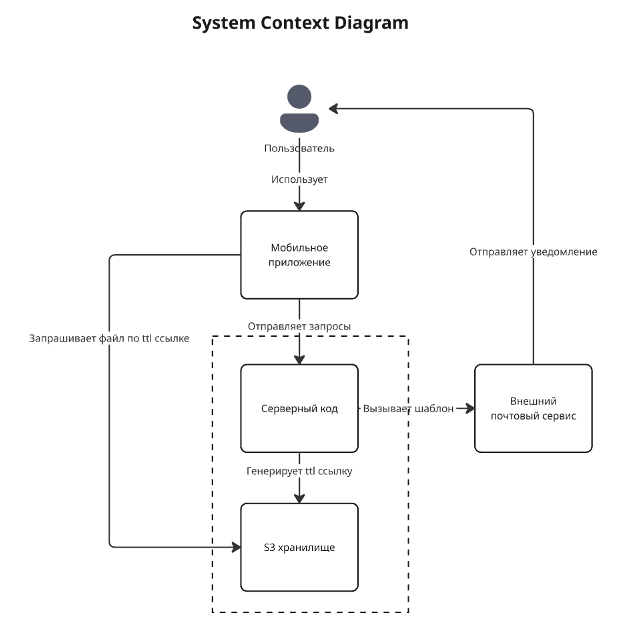
\includegraphics[width=0.8\linewidth]{Images/second_chapter_backend_architecture/Picture1.png}
        \caption{Системная контекстная диаграмма}
        \label{fig:system-context-diagram}
\end{figure}

\subsubsection*{Контейнерная диаграмма}
Контейнерная диаграмма демонстрирует ключевые контейнеры системы и связи между ними. В архитектуре приложения выделены следующие компоненты:
\begin{itemize}
    \item Envoy — обратный прокси/API-шлюз, принимающий все входящие gRPC-запросы и выполняющий маршрутизацию и балансировку нагрузки между сервисами;
    \item Auth Service — сервис аутентификации и авторизации пользователей;
    \item Profile Service — сервис управления профилями пользователей и подписками;
    \item Content Service — сервис управления маршрутами и достопримечательностями;
    \item Activity Service — сервис обработки пользовательской активности (лайки и комментарии);
    \item Notifications Service — сервис отправки уведомлений (email);
    \item FileStorage Service — сервис управления загрузкой и выдачей файлов, генерации временных ссылок (TTL);
    \item Broker Service — служба для маршрутизации и логирования событий между сервисами;
    \item NATS JetStream — брокер сообщений, обеспечивающий асинхронную коммуникацию и передачу событий между сервисами;
    \item PostgreSQL — реляционные базы данных для хранения постоянных данных сервисов;
    \item Redis — кэш и хранилище сессий/токенов;
    \item MinIO (S3-совместимое хранилище) — внешнее файловое хранилище для сохранения медиафайлов.
\end{itemize}
Входящие запросы от мобильного клиента сначала обрабатываются Envoy, который перенаправляет gRPC-вызовы к соответствующим микросервисам и обеспечивает балансировку нагрузки между их инстансами. Микросервисы взаимодействуют между собой синхронно через gRPC-вызовы и асинхронно посредством публикации и подписки на события в NATS JetStream. Таким образом обмен данными организован через комбинацию прямых RPC-вызовов и системы обмена сообщениями.
\begin{figure}[H]
        \centering
        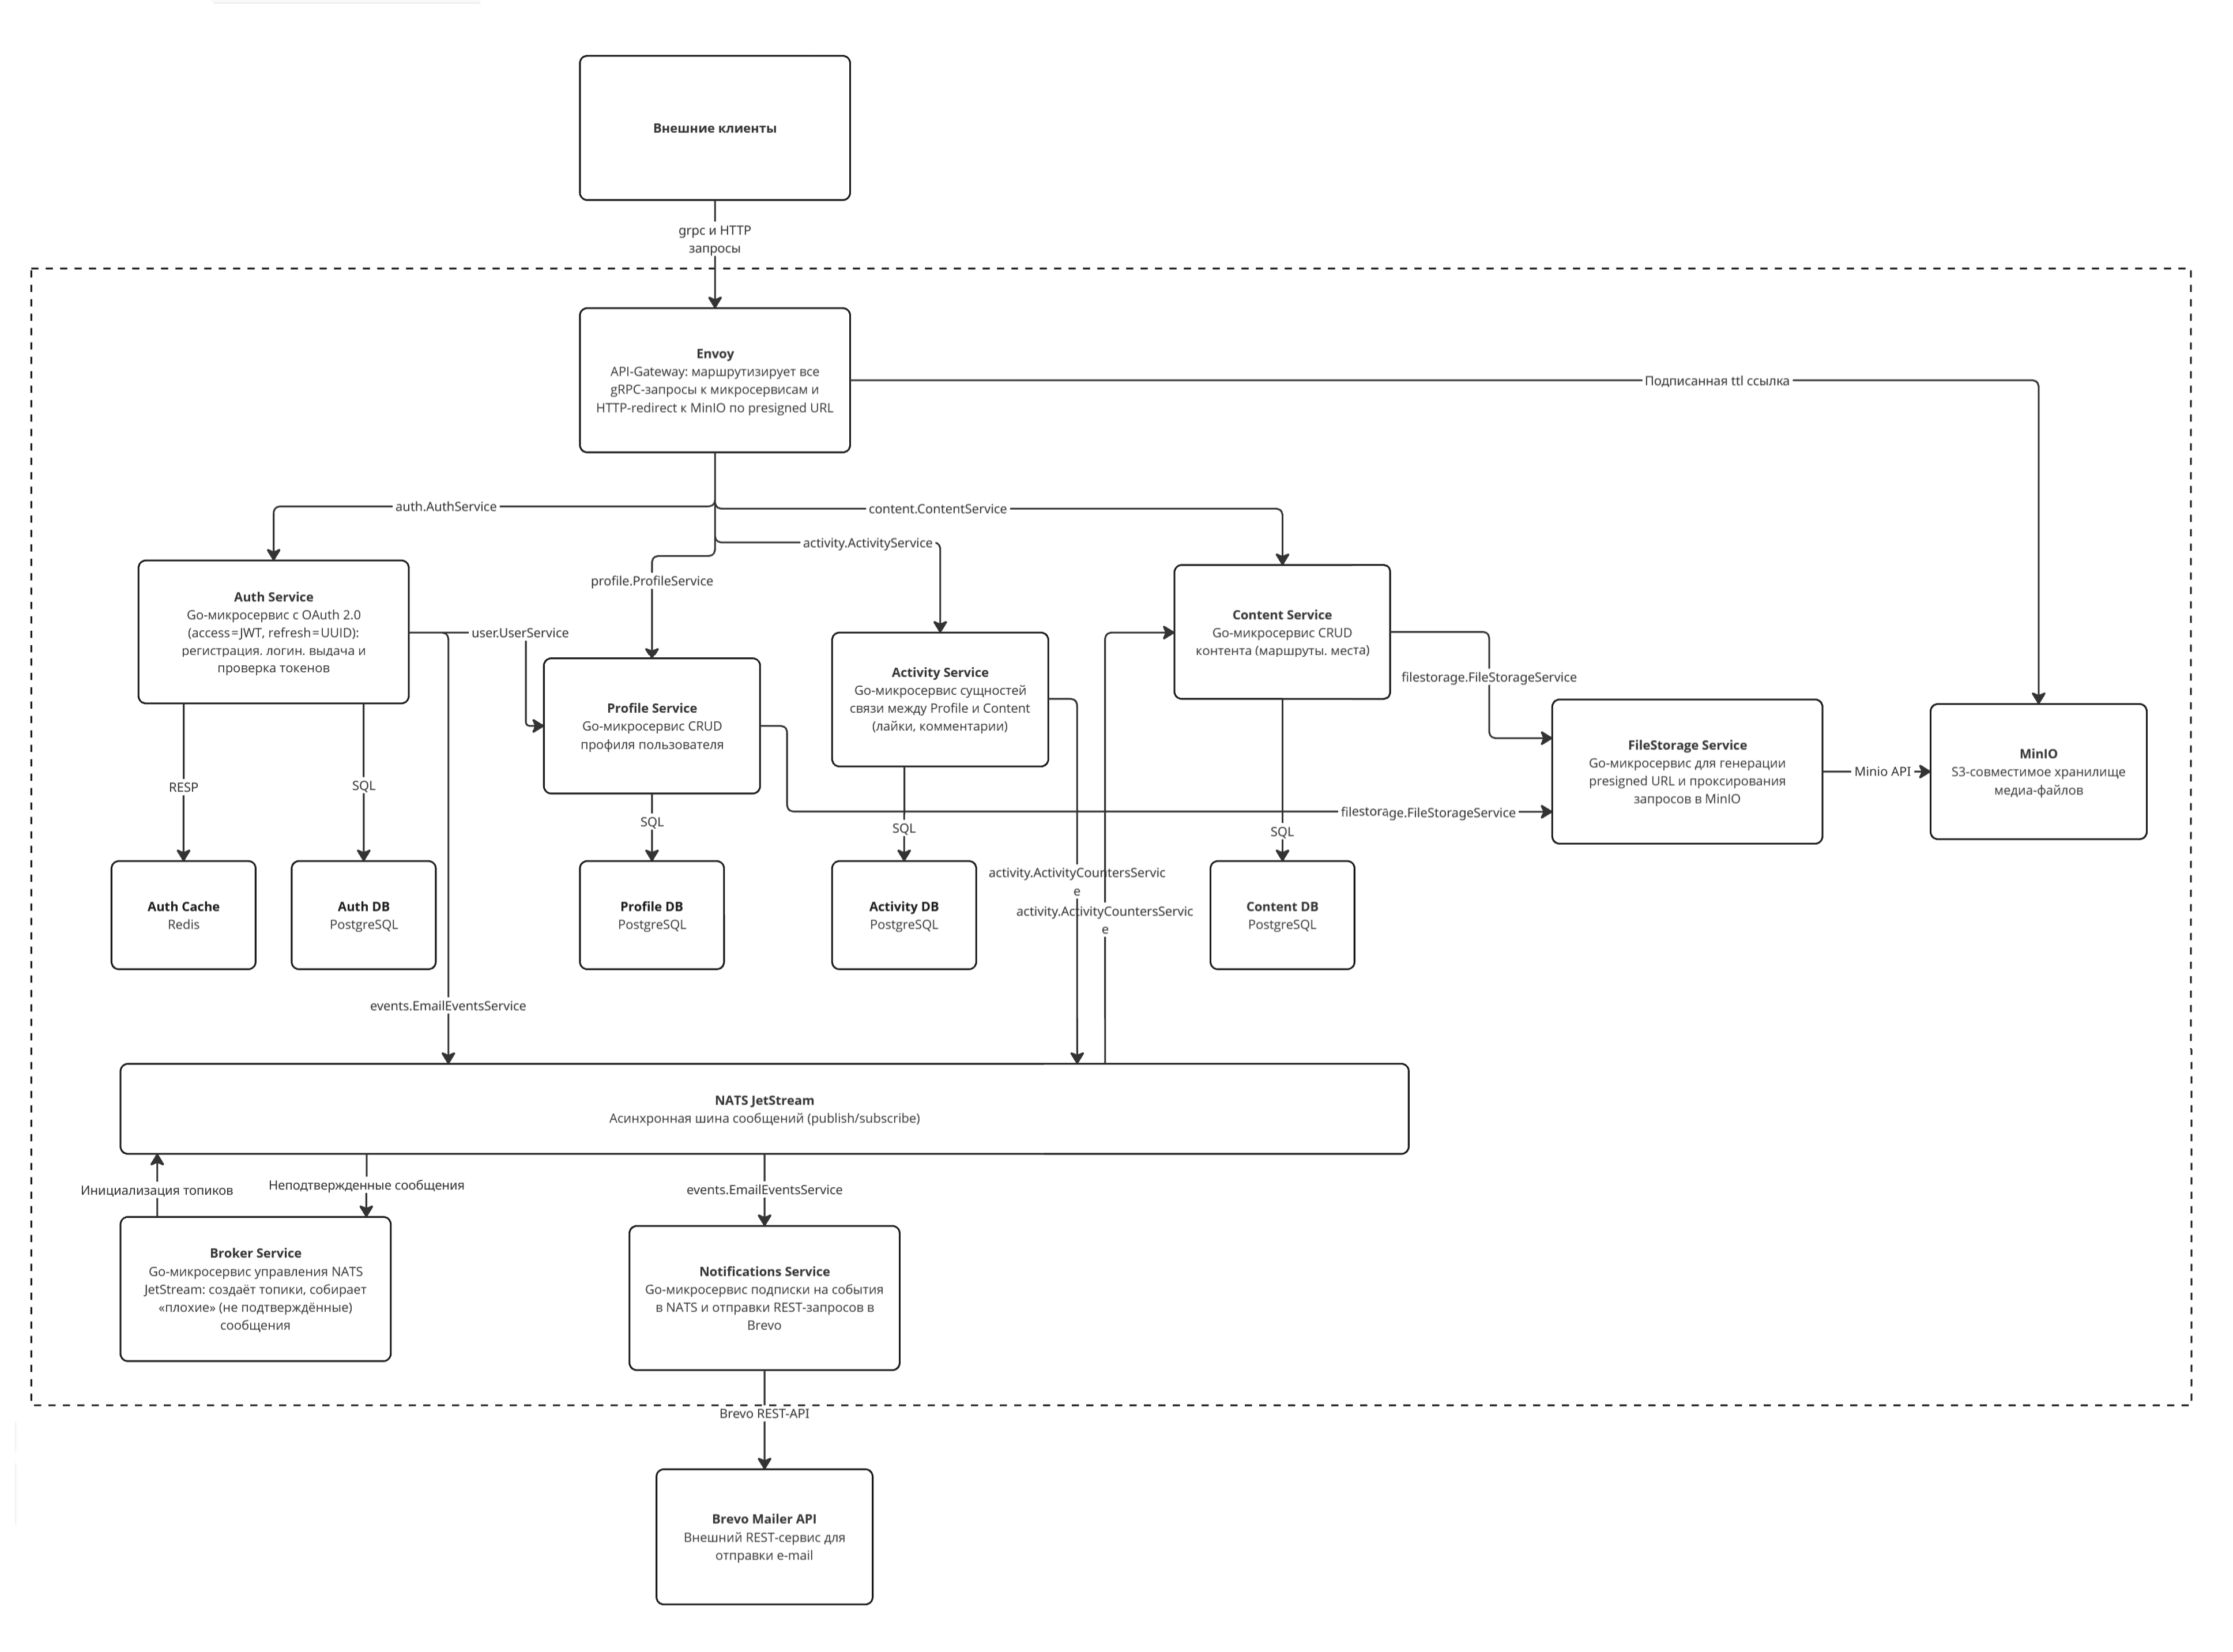
\includegraphics[width=0.8\linewidth]{Images/second_chapter_backend_architecture/Picture2.png}
        \caption{Контейнерная диаграмма}
        \label{fig:container-diagram}
\end{figure}

\subsubsection*{Компонентные диаграммы}
Для каждого микросервиса приведены компонентные диаграммы, описывающие их внутреннюю структуру и основные модули:

\textbf{Auth Service} отвечает за регистрацию и аутентификацию пользователей. В состав сервиса входят следующие компоненты:
\begin{itemize}
    \item Transport (gRPC) — слой транспорта, принимающий входящие gRPC-запросы от Envoy (например, команды регистрации и логина);
    \item User Service — модуль бизнес-логики, управляющий данными пользователей (создание и обновление учетных записей);
    \item Token Service — модуль управления токенами (генерация и проверка JWT или других токенов доступа);
    \item PostgreSQL — реляционная база данных, содержащая таблицу users с полями user\_id (PK, UUID), email, пароль и другими атрибутами учетных записей;
    \item Redis — кэш для хранения активных сессий и токенов доступа (для быстрой проверки валидности токенов);
    \item NATS JetStream — брокер сообщений для публикации событий (например, оповещения других сервисов о регистрации нового пользователя).
\end{itemize}
Сервис выполняет логику авторизации и выдачи токенов, обеспечивает хранение информации о пользователях и токенах, а также публикует события об изменениях в учетных записях.
\begin{figure}[H]
        \centering
        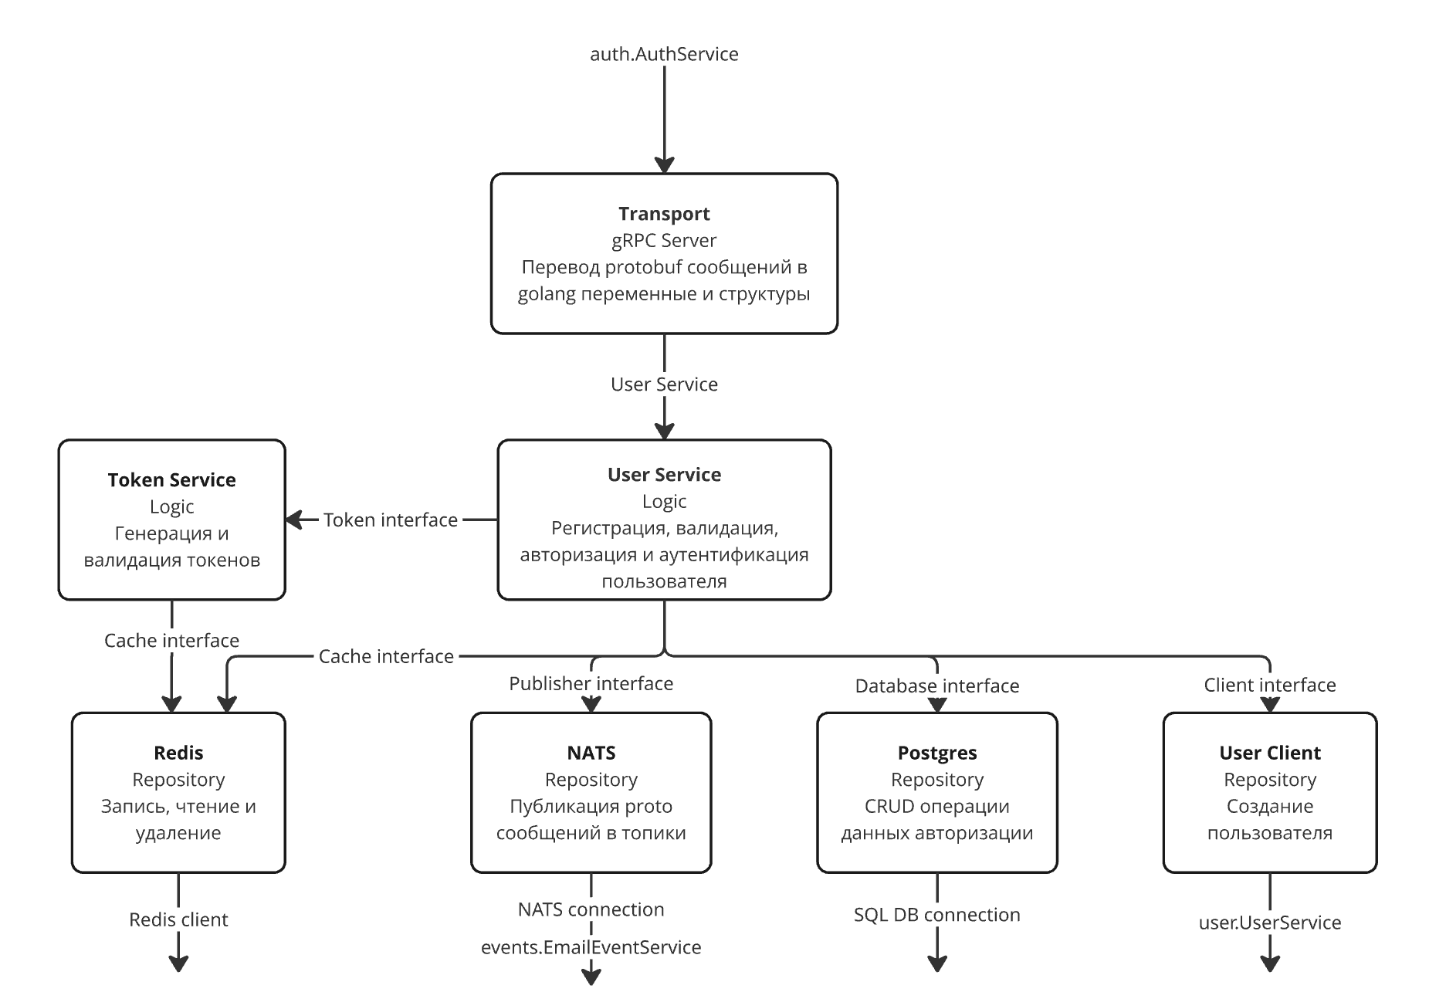
\includegraphics[width=0.8\linewidth]{Images/second_chapter_backend_architecture/Picture3.png}
        \caption{Компонентная диаграмма Auth сервиса}
        \label{fig:auth-service-component-diagram}
\end{figure}

\textbf{Profile Service} управляет информацией профиля пользователя и его социальными связями. В состав микросервиса входят:
\begin{itemize}
    \item Transport (gRPC) — интерфейс приема gRPC-запросов для создания и редактирования профиля, а также управления подписками;
    \item Profile Logic — бизнес-логика сервиса, обрабатывающая операции создания/обновления профиля и управления отношениями «подписка–подписчик»;
    \item PostgreSQL — база данных с таблицами profiles (профили пользователей) и follows (таблица отношений «подписчик–подписка»);
    \item FileStorage Client — клиентский модуль для взаимодействия с FileStorage Service при загрузке аватаров и других файлов профиля.
\end{itemize}
Profile Service позволяет пользователям редактировать свои профили (имя, аватар, информацию о себе) и управлять списками подписок на других пользователей. Компоненты сервиса обеспечивают проверку и запись данных в базу и загрузку файлов аватаров в файловое хранилище.
\begin{figure}[H]
        \centering
        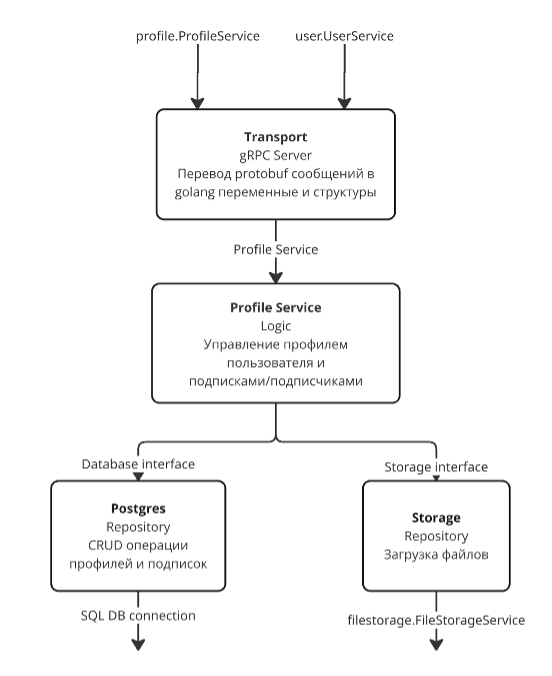
\includegraphics[width=0.8\linewidth]{Images/second_chapter_backend_architecture/Picture4.png}
        \caption{Компонентная диаграмма Profile сервиса}
        \label{fig:profile-service-component-diagram}
\end{figure}

\textbf{Activity Service} отвечает за обработку действий пользователей, связанных с активностью (лайки и комментарии). В составе сервиса выделяются:
\begin{itemize}
    \item Transport (gRPC) — прием и обработка gRPC-запросов типа «добавить лайк» или «оставить комментарий»;
    \item Activity Logic — бизнес-логика, реализующая операции добавления/удаления лайков и комментариев к маршрутам;
    \item PostgreSQL — база данных, содержащая таблицы route\_likes (связка «пользователь–лайк–маршрут») и route\_comments (комментарии к маршрутам);
    \item NATS JetStream — брокер сообщений для публикации событий активности (например, публикация нового комментария может инициировать отправку уведомления другим сервисам).
\end{itemize}
Сервис Activity обрабатывает сохранение лайков и комментариев в базе данных и передает события об этой активности в систему через NATS для дальнейшей обработки (уведомления, статистика и др.).
\begin{figure}[H]
        \centering
        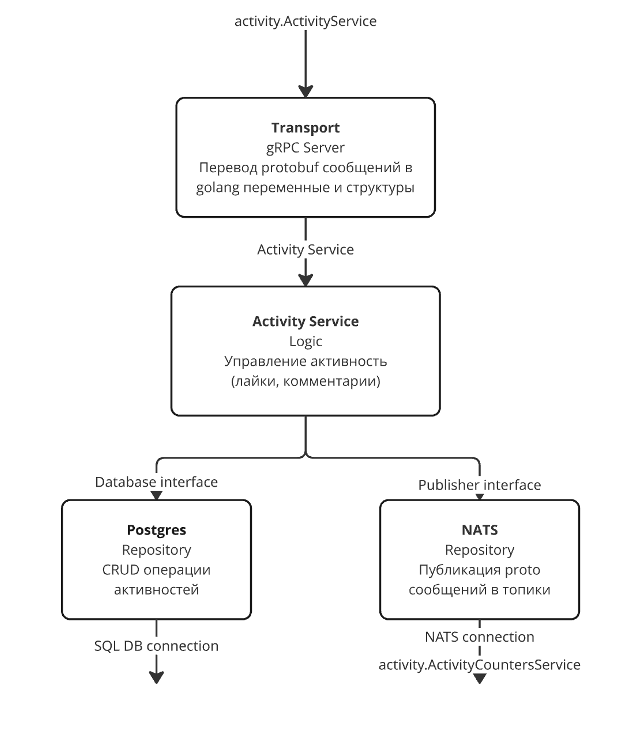
\includegraphics[width=0.8\linewidth]{Images/second_chapter_backend_architecture/Picture5.png}
        \caption{Компонентная диаграмма Activity сервиса}
        \label{fig:activity-service-component-diagram}
\end{figure}

\textbf{Content Service} отвечает за управление основным контентом приложения: маршрутами и достопримечательностями (местами). Компоненты микросервиса включают:
\begin{itemize}
    \item Transport (gRPC) — интерфейс для приема запросов на создание/чтение/обновление/удаление маршрутов и мест;
    \item Content Logic — бизнес-логика для создания, редактирования и удаления маршрутов (routes) и мест (places), а также управления связями между ними;
    \item PostgreSQL — база данных с таблицами routes (маршруты), places (достопримечательности), route\_places (связующая таблица между routes и places), place\_files (связи между places и files).
    \item FileStorage Client — клиент для взаимодействия с FileStorage Service при загрузке файлов (например, изображений) для мест и маршрутов;
    \item NATS Listener — слушатель событий из NATS (например, для отслеживания удалений пользователей или обновлений другого контента).
\end{itemize}
Content Service управляет информацией о туристических маршрутах и местах. Он обеспечивает сохранение метаданных о маршрутах и местах в базе данных и обращение к файловому хранилищу при работе с медиаконтентом.
\begin{figure}[H]
        \centering
        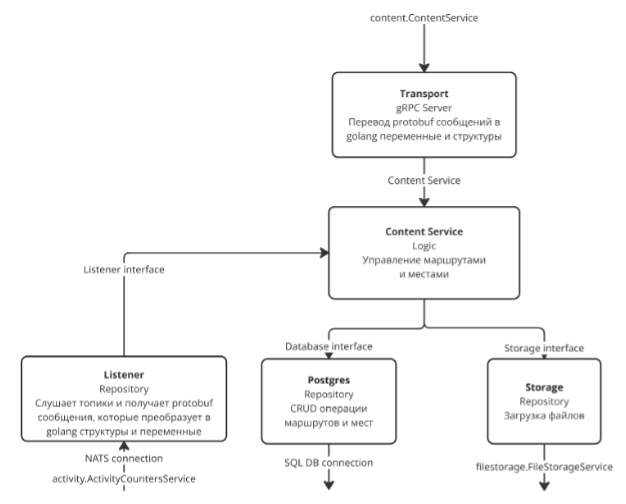
\includegraphics[width=0.8\linewidth]{Images/second_chapter_backend_architecture/Picture6.png}
        \caption{Компонентная диаграмма Content сервиса}
        \label{fig:content-service-component-diagram}
\end{figure}

\textbf{Notifications Service} занимается отправкой email-уведомлений пользователям по различным событиям системы. Компоненты сервиса включают:
\begin{itemize}
    \item Mailer Service — модуль, формирующий и отправляющий электронные письма;
    \item NATS Listener — подписчик на события из NATS JetStream (например, события о регистрации нового пользователя, новом комментарии и др.), инициирующий отправку уведомления;
    \item Внешний почтовый сервис (Brevo API) — сторонний сервис доставки писем.
\end{itemize}
При поступлении события Notifications Service формирует письмо с контентом события и через API внешнего почтового сервиса Brevo отправляет его пользователю. \\ Таким образом реализована асинхронная отправка email-уведомлений по событиям системы.
\begin{figure}[H]
        \centering
        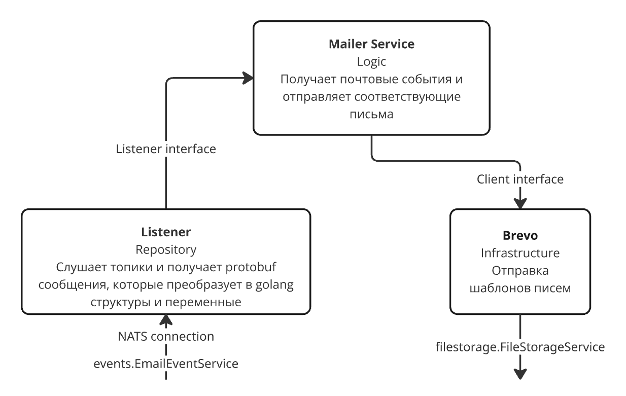
\includegraphics[width=0.8\linewidth]{Images/second_chapter_backend_architecture/Picture7.png}
        \caption{Компонентная диаграмма Notifications сервиса}
        \label{fig:notifications-service-component-diagram}
\end{figure}

\textbf{FileStorage Service} управляет загрузкой и выдачей файлов (например, изображений и других медиа). Его компоненты включают:
\begin{itemize}
    \item Transport (gRPC) — интерфейс приема запросов на загрузку/скачивание файлов;
    \item File Logic — бизнес-логика, генерирующая защищенные временные URL (TTL-ссылки) для операций с файлами, а также обрабатывающая метаданные файлов;
    \item MinIO SDK — библиотека для взаимодействия с S3-совместимым хранилищем MinIO.
\end{itemize}
При получении запроса на загрузку FileStorage Service создает временную ссылку с ограниченным сроком действия, по которой клиент может напрямую передать файл в MinIO. Сервис также может управлять метаданными файлов (имя, тип, размер и др.), сохраняемыми в базе данных. FileStorage Service обеспечивает безопасное и эффективное хранение любых типов файлов, используемых приложением.
\begin{figure}[H]
        \centering
        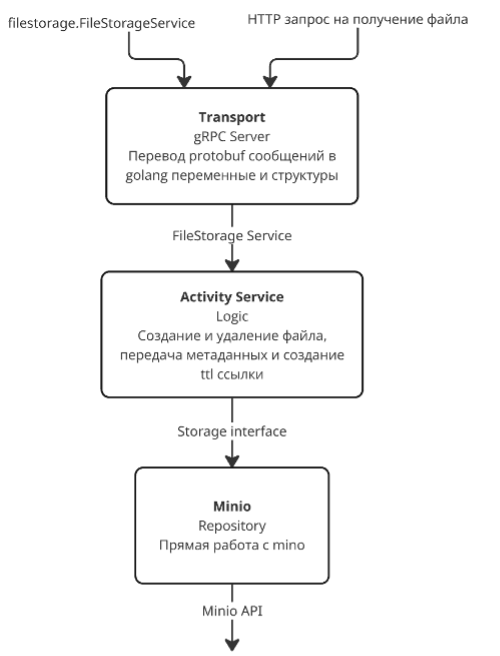
\includegraphics[width=0.8\linewidth]{Images/second_chapter_backend_architecture/Picture8.png}
        \caption{Компонентная диаграмма FileStorage сервиса}
        \label{fig:filestorage-service-component-diagram}
\end{figure}

\textbf{Broker Service} служит для организации обмена сообщениями между микросервисами. Его компоненты включают:
\begin{itemize}
    \item Broker Logic — модуль логики инициализации обмена событиями и логирования;
    \item Listener (NATS) — слушатель, подписанный на необходимые топики в NATS JetStream;
    \item NATS JetStream — система обмена сообщениями, где определены темы (topics) для сервиса.
\end{itemize}
Broker Service отвечает за настройку публикации и маршрутизацию сообщений между сервисами, а также за сбор и логирование событий в системе.
\begin{figure}[H]
        \centering
        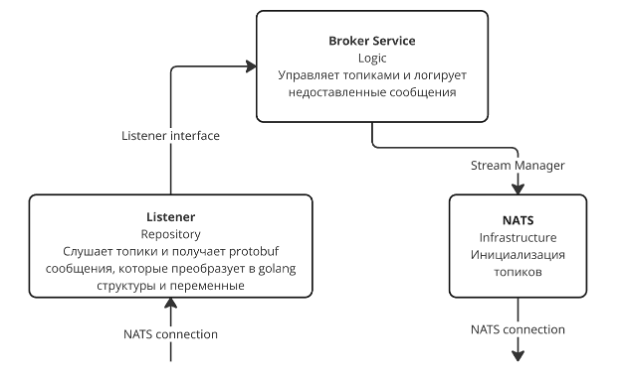
\includegraphics[width=0.8\linewidth]{Images/second_chapter_backend_architecture/Picture9.png}
        \caption{Компонентная диаграмма Broker сервиса}
        \label{fig:broker-service-component-diagram}
\end{figure}

\subsubsection*{ER-диаграммы баз данных}
\textbf{Auth Service:} Сервис аутентификации управляет учётными записями пользователей, обеспечивая регистрацию и авторизацию. В ERD этой системы имеется одна таблица users для хранения базовой информации об учётных записях:
\begin{itemize}
    \item email (text) — адрес электронной почты пользователя; используется для идентификации учётной записи при авторизации. Обычно это логин пользователя в системе.
    \item password (text) — хеш пароля пользователя; хранится в зашифрованном виде для последующей проверки.
    \item status (user\_status) — текущий статус учётной записи; специальный тип (перечисление), задающий состояние пользователя (например, ACTIVE, SUSPENDED и т. п.). Позволяет пометить аккаунт как активный, заблокированный или ожидающий подтверждения.
    \item created\_at (timestamp with time zone) — дата и время создания учётной записи; заполняется автоматически при регистрации пользователя в системе.
    \item updated\_at (timestamp with time zone) — дата и время последнего обновления записи; обновляется при изменении данных пользователя.
    \item id (uuid, PRIMARY KEY) — глобально уникальный идентификатор пользователя; первичный ключ таблицы. Используется для однозначной связи пользователя между всеми сервисами системы.
\end{itemize}
Стоит отметить, что uuid применяется во всех таблицах нашей системы в качестве глобального уникального идентификатора. Например, поле id в таблице users имеет тип uuid и связывает данные из этого сервиса с другими микросервисами через единый идентификатор пользователя.
\begin{figure}[H]
        \centering
        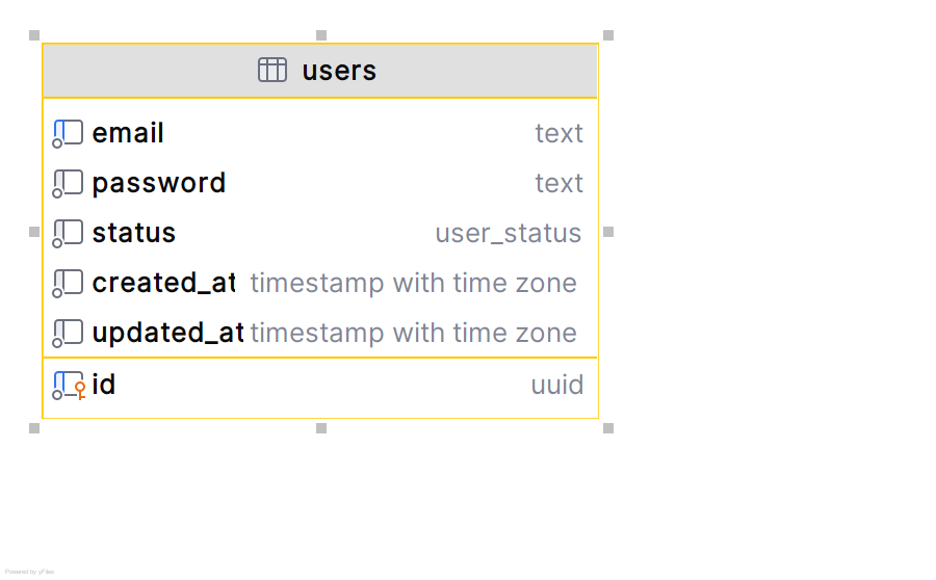
\includegraphics[width=0.8\linewidth]{Images/second_chapter_backend_architecture/Picture10.png}
        \caption{ERD Auth сервиса}
        \label{fig:auth-service-erd}
\end{figure}

\textbf{Profile Service:} Сервис профилей хранит дополнительную информацию о пользователе, не связанную непосредственно с учётными данными, а также информацию о связях «подписчиков-подписок». ERD этого сервиса включает следующие таблицы:

Таблица profiles содержит персональные данные пользователя и его статистику подписок:
\begin{itemize}
    \item username (text) — уникальное имя пользователя в системе (никнейм); служит для отображения в интерфейсе и может использоваться при поиске.
    \item first\_name (text) — имя пользователя; хранится для отображения полного имени в профиле.
    \item last\_name (text) — фамилия пользователя; аналогично отображается в профиле.
    \item date\_of\_birth (date) — дата рождения; может использоваться для определения возраста и персонализации.
    \item followers\_count (integer) — количество подписчиков (followers) данного профиля; поле для быстрого доступа к этой статистике.
    \item image\_id (integer, FOREIGN KEY) — ссылка на файл с аватаром пользователя; внешний ключ, ссылающийся на поле id таблицы files (сервиса FileStorage). Хранит идентификатор файла-аватара в файловом хранилище.
    \item created\_at (timestamp with time zone) — дата и время создания профиля (обычно совпадает с регистрацией); автоматически задаётся при инициации профиля.
    \item updated\_at (timestamp with time zone) — дата и время последнего обновления профиля (например, после изменения имени или фото).
    \item following\_count (integer) — количество пользователей, на которых подписан данный пользователь; поле для быстрого отображения статистики «подписок».
    \item user\_id (uuid, PRIMARY KEY, FOREIGN KEY) — глобально уникальный идентификатор пользователя; первичный ключ таблицы profiles. Кроме того, это внешний ключ на таблицу users сервиса Auth и указывает на соответствующую учётную запись пользователя.
\end{itemize}
Таблица follows фиксирует отношения подписки между пользователями («кто на кого подписался»):
\begin{itemize}
    \item created\_at (timestamp with time zone) — дата и время установления подписки; автоматически задаётся при создании записи подписки.
    \item followed\_id (uuid, PRIMARY KEY (совместно с follower\_id), FOREIGN KEY) — идентификатор пользователя, на которого осуществлена подписка. Является частью составного первичного ключа и внешним ключом на поле user\_id таблицы profiles (или users сервиса Auth).
    \item follower\_id (uuid, PRIMARY KEY (совместно с followed\_id), FOREIGN KEY) — идентификатор пользователя, совершившего подписку (подписчика). Также часть составного первичного ключа и внешний ключ на user\_id таблицы profiles.
\end{itemize}
Таким образом, составной ключ (follower\_id, followed\_id) гарантирует уникальность каждой пары «подписчик–подписка», а оба поля ссылаются на записи пользователей. Данная таблица не содержит отдельного идентификатора (ID), так как уникальность обеспечивается комбинацией этих двух полей.

Основные поля таблицы files следующие:
\begin{itemize}
    \item file\_name (text) — исходное имя файла при загрузке. Сохраняется для информационных целей (например, отображение названия).
    \item storage\_bucket (text) — имя хранилища или «бакета» в облачном хранилище (например, S3), где находится файл.
    \item storage\_id (text) — внутренний идентификатор файла в хранилище (например, ключ объекта); используется для извлечения файла из облака.
    \item internal\_url (text) — сгенерированный URL или путь для доступа к файлу внутри системы (например, через CDN или сервер файлов); может использоваться для получения файла.
    \item placeholder (text) — данные-заполнитель или URL для превью/миниатюры файла; может содержать ссылку на уменьшенное изображение или другой вспомогательный контент.
    \item created\_at (timestamp with time zone) — дата и время добавления файла в систему; автоматически фиксируется при загрузке файла.
    \item from\_public (boolean) — флаг, указывающий, был ли файл получен из публичного источника. Например, true — файл взят из публичной ссылки, false — загружен через приложение.
    \item size (bigint) — размер файла в байтах; хранится для контроля и статистики использования пространства.
    \item id (integer, PRIMARY KEY) — уникальный идентификатор файла; первичный ключ таблицы files.
\end{itemize}
Таблица files используется не только для хранения изображений (аватаров, фото мест и т. д.), но и для любых других файлов, необходимых системе.
\begin{figure}[H]
        \centering
        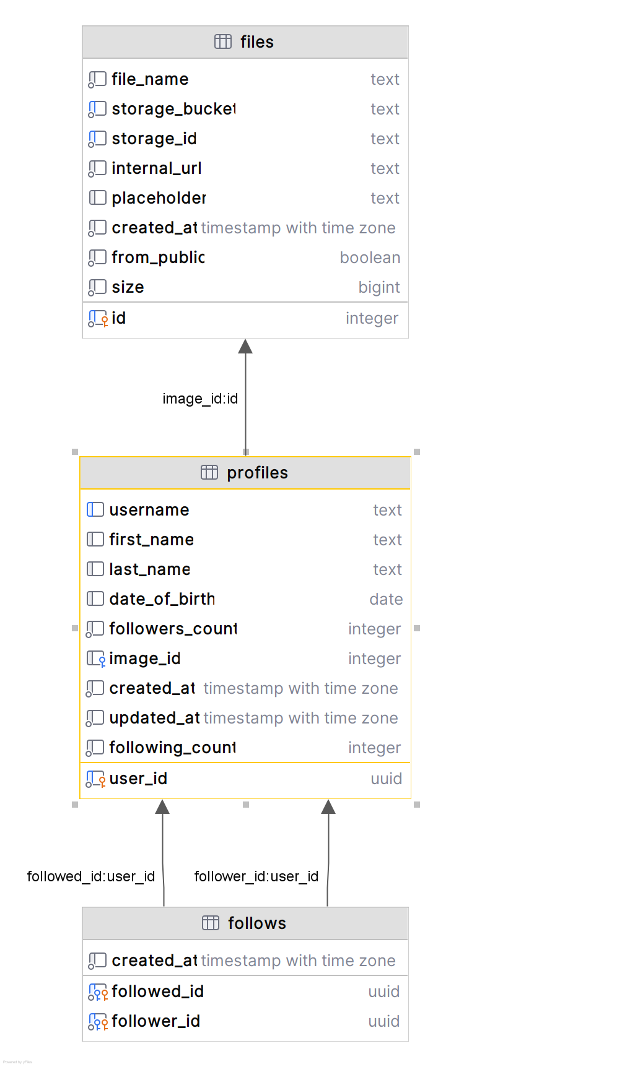
\includegraphics[width=0.8\linewidth]{Images/second_chapter_backend_architecture/Picture11.png}
        \caption{ERD Profile сервиса}
        \label{fig:profile-service-erd}
\end{figure}

\textbf{Content Service:} Сервис контента управляет информацией о туристических маршрутах и местах. ERD этого сервиса состоит из следующих таблиц:

Таблица routes содержит описание путешествий-туров:
\begin{itemize}
    \item name (text) — название маршрута; краткое описание, которое видит пользователь.
    \item difficulty (difficulty\_level) — уровень сложности маршрута; специальный перечислимый тип (enum), задающий категорию сложности (например, EASY, MODERATE, HARD).
    \item distance (real) — протяжённость маршрута (например, в километрах); числовое поле с плавающей точкой.
    \item user\_id (uuid, FOREIGN KEY) — идентификатор пользователя, создавшего маршрут; \\ внешний ключ на таблицу users сервиса Auth (или profiles.user\_id). Позволяет связать маршрут с автором.
    \item latitude (double precision[]) — массив значений широт точек маршрута; используется для хранения многоугольника пути (географические координаты всех точек маршрута).
    \item longitude (double precision[]) — массив долготы точек маршрута; параллельно latitude описывает путь.
    \item created\_at (timestamp with time zone) — дата и время создания маршрута; автоматически присваивается при добавлении нового маршрута.
    \item updated\_at (timestamp with time zone) — дата и время последнего изменения маршрута (например, после редактирования описания или пути).
    \item description (text) — подробное текстовое описание маршрута; может включать рекомендации, обзор мест.
    \item id (uuid, PRIMARY KEY) — глобально уникальный идентификатор маршрута; первичный ключ таблицы routes.
\end{itemize}
Таблица places содержит информацию о конкретных местах (точках интереса):
\begin{itemize}
    \item name (text) — название места (например, название достопримечательности или географического объекта).
    \item address (text) — адрес или описание местоположения места (улица, город и т. п.).
    \item description (text) — детальное описание места; история, примечания, другая справочная информация.
    \item latitude (double precision) — широта географического расположения места (одиночная координата).
    \item longitude (double precision) — долгота географического расположения места.
    \item created\_at (timestamp with time zone) — дата и время добавления записи о месте; автоматически заполняется при создании.
    \item updated\_at (timestamp with time zone) — дата и время последнего обновления данных места.
    \item id (uuid, PRIMARY KEY) — глобально уникальный идентификатор места; первичный ключ таблицы places.
\end{itemize}
Таблица route\_places связывает маршруты и места, формируя последовательность точек маршрута:
\begin{itemize}
    \item route\_id (uuid, FOREIGN KEY) — идентификатор маршрута; внешний ключ на id таблицы routes.
    \item place\_id (uuid, FOREIGN KEY) — идентификатор места; внешний ключ на id таблицы places.
    \item ordering (integer) — порядок (позиция) места в данном маршруте; указывает, в каком порядке пользователь посещает эти места.
    \item id (integer, PRIMARY KEY) — уникальный идентификатор записи; первичный ключ таблицы.
\end{itemize}
Данная таблица реализует связь «многие-ко-многим» между маршрутами и местами, причём через поле ordering поддерживается упорядоченность. Каждая запись указывает, что конкретное место входит в маршрут.

Таблица place\_files хранит связь между местами и файлами (например, фотографиями мест):
\begin{itemize}
    \item ordering (integer) — порядок файла в списке файлов для данного места; помогает упорядочить изображения.
    \item place\_id (uuid, FOREIGN KEY) — идентификатор места; внешний ключ на id таблицы places.
    \item file\_id (integer, FOREIGN KEY) — идентификатор файла; внешний ключ на id таблицы files сервиса FileStorage.
    \item id (integer, PRIMARY KEY) — уникальный идентификатор записи; первичный ключ таблицы place\_files.
\end{itemize}
Таким образом, таблица place\_files связывает множество файлов с каждым местом, позволяя прикреплять к месту изображения и другие медиафайлы. Для каждого связанного файла хранится его сортировочный индекс (ordering) и ссылки на место и файл.
Таблица files аналогична одноименной таблице из Profile сервиса.
\begin{figure}[H]
        \centering
        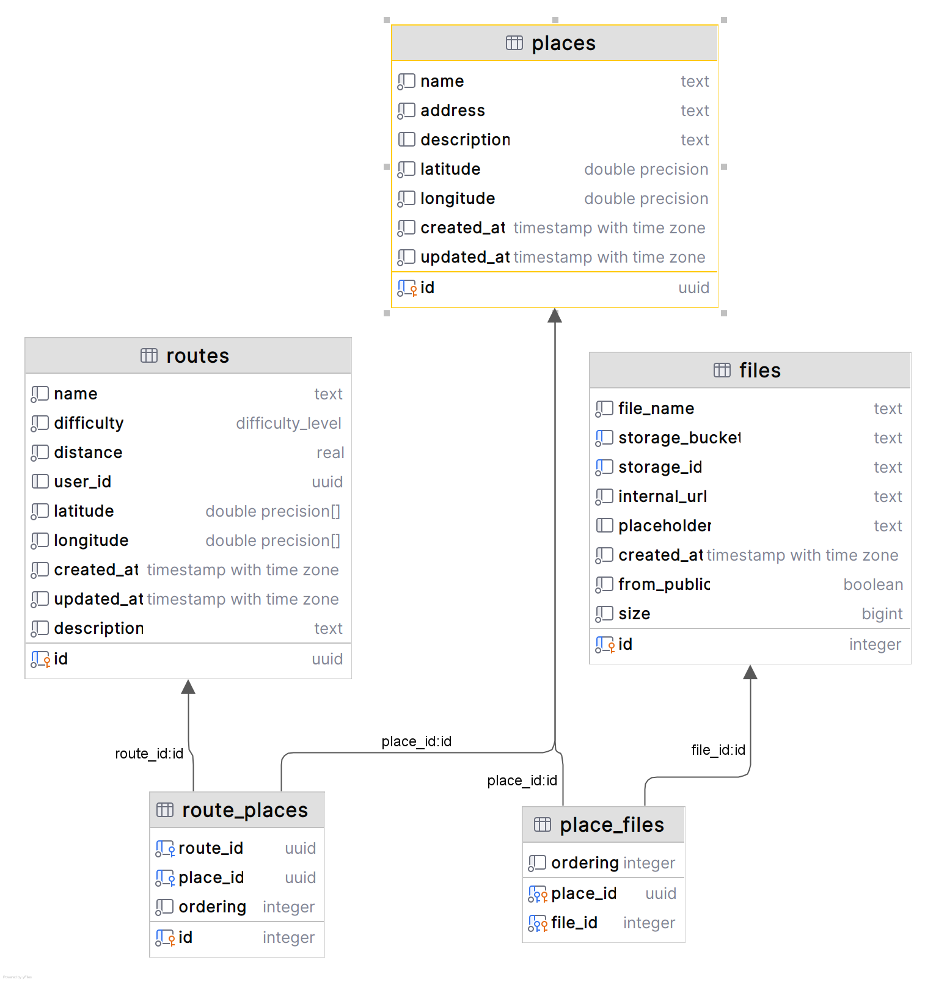
\includegraphics[width=0.8\linewidth]{Images/second_chapter_backend_architecture/Picture12.png}
        \caption{ERD Content сервиса}
        \label{fig:content-service-erd}
\end{figure}

\textbf{Activity Service:} Сервис активности отвечает за пользовательские взаимодействия с маршрутами — лайки и комментарии. ERD этого сервиса включает следующие таблицы:
Таблица route\_likes фиксирует факт постановки лайка маршруту:
\begin{itemize}
    \item created\_at (timestamp with time zone) — дата и время проставления лайка; автоматически устанавливается при создании записи.
    \item route\_id (uuid, PRIMARY KEY (вместе с user\_id), FOREIGN KEY) — идентификатор маршрута, которому поставлен лайк; внешний ключ на id таблицы routes. Является частью составного первичного ключа вместе с user\_id.
    \item user\_id (uuid, PRIMARY KEY (вместе с route\_id), FOREIGN KEY) — идентификатор пользователя, поставившего лайк; внешний ключ на таблицу users (или profiles.user\_id). Является частью составного первичного ключа.
\end{itemize}
Комбинация полей (route\_id, user\_id) образует составной первичный ключ, что гарантирует, что каждый пользователь может поставить лайк заданному маршруту не более одного раза. Таким образом эта таблица не имеет отдельного ID.

Таблица route\_comments хранит комментарии пользователей к маршрутам:
\begin{itemize}
    \item route\_id (uuid, FOREIGN KEY) — идентификатор маршрута, к которому оставлен комментарий; внешний ключ на id таблицы routes.
    \item user\_id (uuid, FOREIGN KEY) — идентификатор пользователя, написавшего комментарий; внешний ключ на таблицу users.
    \item text (text) — текст комментария.
    \item created\_at (timestamp with time zone) — дата и время публикации комментария.
    \item comment\_id (bigint, PRIMARY KEY) — уникальный идентификатор комментария; первичный ключ таблицы route\_comments.
\end{itemize}
Поле comment\_id является автоинкрементным или генерируется последовательно и гарантирует уникальность комментария. Остальные поля связывают комментарий с маршрутом и пользователем.
\begin{figure}[H]
        \centering
        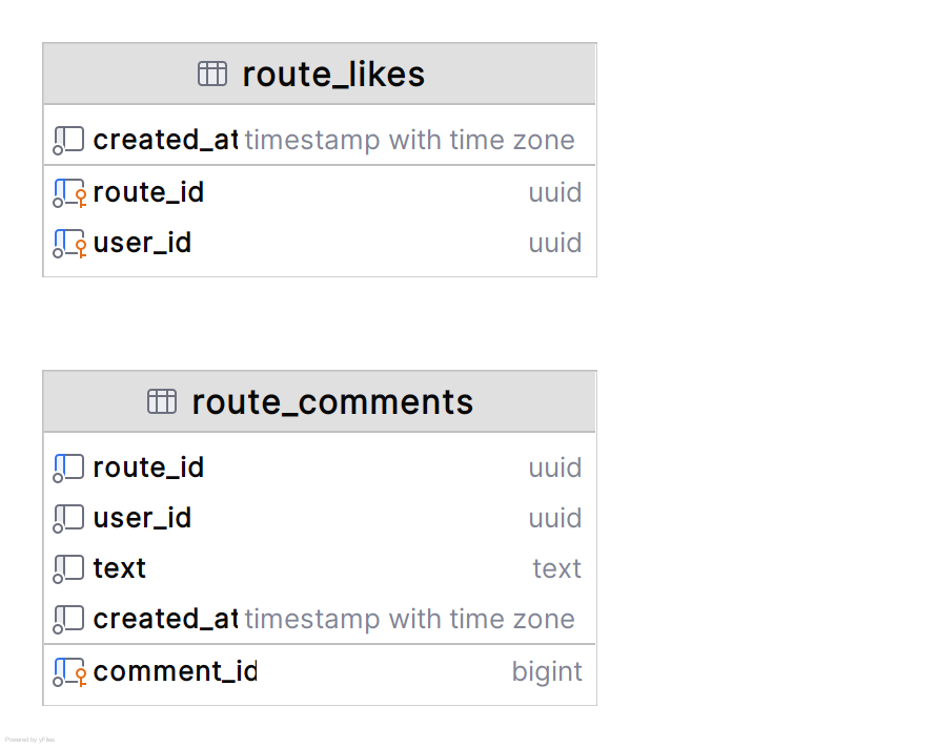
\includegraphics[width=0.8\linewidth]{Images/second_chapter_backend_architecture/Picture13.png}
        \caption{ERD Activity сервиса}
        \label{fig:activity-service-erd}
\end{figure}

\subsection*{2.4 Компоненты инфраструктуры}
\addcontentsline{toc}{subsection}{2.4 Компоненты инфраструктуры}
Организация инфраструктуры и DevOps-процессов является важной частью проектирования микросервисной системы приложения «Путешествия по России». На этапе проектирования проекта принимаются решения о средствах автоматизации сборки, тестирования и развертывания, а также о способах управления артефактами и конфигурациями. В данном разделе описываются основные компоненты инфраструктуры: процесс CI/CD на основе GitHub Actions, использование \\ GitHub Container Registry для хранения артефактов, система Helm-чартов для управления развертыванием, балансировка нагрузки через Envoy и подходы к хранению конфигураций и секретов.

\subsubsection*{CI/CD-процесс на основе GitHub Actions}
Для обеспечения непрерывной интеграции и доставки (CI/CD) в микросервисной архитектуре приложения «Путешествия по России» на этапе проектирования предусматривается использование платформы GitHub Actions. Проект состоит из множества независимых репозиториев, соответствующих отдельным микросервисам (например, vkr-auth, vkr-notifications, vkr-profile и др.). В каждом репозитории настраивается собственный workflow в GitHub Actions, реализующий этапы сборки и доставки сервисов. При каждом пуше в ветку main запускается автоматизированный процесс сборки: если изменяется код микросервиса, запускается создание Docker-образа этого сервиса и его публикация в \\ GitHub Container Registry (GHCR); если меняются компоненты платформы, инициируется сборка обновлённого Helm-чарта. Предусматривается отдельный триггер для миграций базы данных: при изменении файлов миграции запускается выполнение соответствующего workflow для применения новых изменений в структуре БД.
Таким образом, внедрение GitHub Actions обеспечивает автоматическое прохождение всего цикла разработки — от фиксации изменений в репозитории до развертывания обновлённой версии приложения. Данный подход исключает необходимость ручного развёртывания и ускоряет выпуск новых версий. В частности, после успешного пуша в главную ветку репозитория vkr-platform, содержащего интегрированный Helm-чарт всех сервисов, в продакшн-окружении автоматически запускается обновление приложений до новой версии.

\subsubsection*{GitHub Container Registry (GHCR)}
В качестве централизованного хранилища контейнерных образов и Helm-чартов в проекте предполагается использовать GitHub Container \\ Registry (GHCR) под личной учётной записью pedrecho. Все образы сервисов и сформированные чарты публикуются в этот регистр, что позволяет удобно управлять версиями артефактов и обеспечивать их доступность при развертывании.
Каждый образ или чарт получает уникальный тег, отражающий версию и дату сборки (например, для чарта используется префикс chart-), при этом предыдущие версии не удаляются из регистра во избежание потери истории и возможности отката. Для аутентификации при публикации и загрузке артефактов в GitHub Container Registry в CI/CD-пайплайнах используются защищённые переменные окружения: GHCR\_USERNAME, GHCR\_TOKEN (токен доступа к регистру) и GOPRIVATE\_PAT (личный токен доступа для приватных Go-модулей). Использование централизованного регистра упрощает управление зависимостями и обеспечивает постоянный доступ к нужным версиям контейнеров и чартов в процессе развертывания.

\subsubsection*{Helm Charts для управления развертываниями}
Для каждого микросервиса разрабатывается собственный Helm-чарт, описывающий его шаблоны развёртывания, сервисы и другие необходимые Kubernetes-ресурсов. В проекте vkr-platform создаётся объединённый («собирательный») Helm-чарт, в котором в качестве зависимостей перечислены все чарты микросервисов и шаблон Envoy, выступающий в роли маршрутизатора. Такой подход позволяет централизовать описание всей системы и обеспечить согласованность версий сервисов при развертывании.
В процессе CI/CD каждый Helm-чарт упаковывается в архив (файл .tgz), затем включается в контейнерный образ или публикуется в реестр артефактов с помощью GitHub Actions. Публикация чарта позволяет Kubernetes-кластеру автоматически получать актуальные сведения о конфигурации сервисов. Это обеспечивает удобную дистрибуцию чартов и автоматическую доставку обновлённых версий конфигураций кластеру при каждой сборке проекта.

\subsubsection*{Балансировка нагрузки и маршрутизация трафика}
В качестве внешнего прокси-сервера и балансировщика нагрузки для gRPC-трафика от мобильного приложения к микросервисам используется \\ Envoy. Все входящие запросы от клиента маршрутизируются через единый контейнер Envoy, что упрощает управление коммуникацией между сервисами и позволяет централизованно настраивать правила маршрутизации. Envoy развёртывается как часть платформенного Helm-чарта и размещается в том же \\ namespace, что и остальные сервисы приложения.
Конфигурация Envoy задаётся с помощью шаблонов Helm и генерируется на основе значений из файлов values.yaml. Такой подход позволяет адаптировать параметры прокси-сервера под различные окружения и случаи использования без изменения исходного кода. При этом система изначально не предполагает использование TLS для межсервисного взаимодействия, поэтому соответствующие настройки шифрования в данном разделе не рассматриваются.

\subsubsection*{Хранение конфигураций и секретов}
Управление конфигурацией системы осуществляется через файлы Helm-чартов values.yaml и values.secret.yaml. В файле values.yaml задаются общие параметры для каждого сервиса, включая настройки подключения, порты и т.д. Файл values.secret.yaml предназначен для конфиденциальных данных (пароли, токены и т.п.), поэтому он не хранится в системе контроля версий. Вместо этого в репозитории сохраняется шаблон \\ values.secret.example.yaml, который иллюстрирует необходимые поля для секретной конфигурации без реальных значений. На этапе деплоя значения из values.yaml и values.secret.yaml компонуются, а соответствующие параметры записываются в объекты \\ ConfigMap и Secret Kubernetes \cite{3}\cite{4}. В Go-приложениях используется единый YAML-файл конфигурации, который формируется из этих значений: переменные окружения подставляются в шаблон Go-конфига на основе собранных данных Helm-чартов. Таким образом, каждый сервис получает все необходимые настройки из одного объединённого YAML-файла, обеспечивая унифицированный и прозрачный механизм конфигурации приложений.

\subsection*{2.5 Меры обеспечения безопасности}
\addcontentsline{toc}{subsection}{2.5 Меры обеспечения безопасности}

\subsubsection*{OAuth 2.0 и Auth Gateway}
Принята модель авторизации OAuth 2.0. При этом выдаётся два вида токенов:
\begin{itemize}
    \item Access-токен (JWT) \cite{7} с коротким временем жизни (около 15 минут).
    \item Refresh-токен (UUID) со значительно более длительным временем жизни (около 7 дней).
\end{itemize}
Для повышения безопасности при выдаче токенов учитывается уникальный «отпечаток» (fingerprint) устройства или браузера пользователя, что привязывает токен к конкретному клиенту. Проверка валидности токенов и их обновление централизованы в сервисе AuthService: у него имеется специальный gRPC-эндпоинт для проверки токенов. Такой подход позволяет гарантировать консистентность управления токенами в системе и повышает надёжность авторизации.

\subsubsection*{Безопасность межсервисного взаимодействия}
Коммуникация между микросервисами осуществляется по внутренним защищённым каналам (через протокол gRPC), проксируемым Envoy. Envoy выступает в роли «data plane» для микросервисов, централизованно управляя трафиком и повышая безопасность сетевого взаимодействия. Кроме того, используются механизмы сегментации сети: сервисы развёрнуты в отдельных namespace Kubernetes, а маршруты между ними ограничены сетевыми политиками (Network Policy). Это минимизирует «боковое» распространение атаки и снижает зону потенциального поражения в случае компрометации отдельного компонента.

\subsubsection*{Шифрование и безопасное хранение данных}
При работе с учётными данными пользователей пароли никогда не сохраняются в открытом виде: перед записью в базу они хэшируются с помощью алгоритма bcrypt. Остальные чувствительные данные пользователей не шифруются явно на уровне приложения, но передаются по защищённым внутренним каналам (TLS внутри кластера) и хранятся в приватных базах данных, доступ к которым строго ограничен. Защита данных на уровне хранилища обеспечивается использованием защищённых томов (PVC). Современные облачные платформы обычно поддерживают автоматическое шифрование томов на уровне хоста или инфраструктуры: например, в GKE on Azure тома данных по умолчанию шифруются платформенными ключами (Azure Key Vault). Это гарантирует, что даже при физическом доступе к носителю данные останутся зашифрованными.

\subsubsection*{Безопасность файлового хранилища}
Хранилище объектов MinIO настроено с разграничением доступа: один публичный бакет используется для общедоступных ресурсов (аватары пользователей, изображения маршрутов и т.п.), тогда как все прочие файлы хранятся в приватных бакетах. Доступ к приватным файлам возможен только по заранее сгенерированным временным URL (pre-signed URL) с ограниченным сроком действия. Такие ссылки действуют строго ограниченное время – после истечения TTL доступ по ним автоматически прекращается. Таким образом, даже при потенциальной утечке ссылки её сила быстро аннулируется, что значительно повышает безопасность файлового хранилища.

\subsubsection*{Резервное копирование и аудит}
Предусмотрено регулярное резервное копирование конфигураций и данных. В частности, современные облачные СУБД и сервисы поддерживают автоматическое ежедневное создание резервных копий – например, в Cloud SQL для MySQL ежедневно выполняется автоматическая резервная копия данных. Хотя конкретный провайдер на этапе проектирования ещё не выбран, в большинстве решений можно настроить автоматическое хранение истории бэкапов с возможностью восстановления. Аудит безопасности реализуется через сбор системных логов на уровне Kubernetes-подов и сервисов. В текущей архитектуре отдельного агрегатора логов нет, но логи формируются последовательно и структурировано, что позволяет в будущем легко подключить централизованные системы мониторинга и аудита (Grafana Loki, ELK и т. п.) для глубокого анализа событий и инцидентов.

\subsection*{Выводы по главе}
\addcontentsline{toc}{subsection}{Выводы по главе}
Проведённый в этой главе анализ и проектирование подтвердили обоснованность выбора микросервисной архитектуры как базового подхода к построению серверной части приложения «Путешествия по России». Предложенная структура — разделение функциональности на независимые сервисы Auth, Profile, Content, Activity, FileStorage и Notifications, взаимодействующие через gRPC и асинхронный брокер NATS JetStream, — обеспечивает требуемые нефункциональные характеристики: масштабируемость (горизонтальное масштабирование отдельных узких мест), отказоустойчивость (локализация сбоев и автоматический перезапуск контейнеров) и гибкость развития (возможность добавления новых доменных сервисов без переработки существующего кода). Детализированные контекстная, контейнерная и компонентные диаграммы визуально подтвердили согласованность слоёв, а ER модели баз данных показали целостность схем хранения, поддерживающих концепцию «база на сервис» и разграничение ответственности за данные.
Важной частью проекта стало описание DevOps инфраструктуры и мер безопасности: автоматизированные CI/CD конвейеры на GitHub Actions, хранение артефактов в GHCR, единый Helm чарт «platform» для развёртывания, балансировка и маршрутизация трафика через Envoy, а также комплекс защитных механизмов (OAuth 2.0, bcrypt хеширование паролей, параметризованные SQL запросы, TTL ссылки на файлы, сегментация сети внутри кластера). Принятые решения гарантируют последовательную доставку изменений в Kubernetes кластер, безопасное хранение чувствительных данных и строгий контроль доступа к ресурсам. Таким образом, в этой главе сформирована целостная и технически обоснованная архитектура, которая служит прочным фундаментом для реализации и последующей эксплуатации системы, соответствуя как функциональным, так и нефункциональным требованиям, выявленным на предыдущем этапе работы.

